\documentclass{article} % Document type 
\usepackage{graphicx} % To include pictures 
\usepackage{url} % Url tag used for links in bibliography 
\graphicspath{{Images/}} % Image path 
\usepackage[nottoc,numbib]{tocbibind} % Bibliography in table of contents 
\usepackage[toc,page]{appendix} % Appendix in table of contents 
\usepackage{listings} % Rest used to include Java code snippets 
\usepackage{minted} % Code Syntax Highlighter 
\usepackage{color}
\definecolor{dkgreen}{rgb}{0,0.6,0}
\definecolor{gray}{rgb}{0.5,0.5,0.5}
\definecolor{mauve}{rgb}{0.58,0,0.82}
 
% Java Code Setup 
 
\lstset{frame=tb,
  language=Java,
  aboveskip=3mm,
  belowskip=3mm,
  showstringspaces=false,
  columns=flexible,
  basicstyle={\small\ttfamily},
  numbers=none,
  numberstyle=\tiny\color{gray},
  keywordstyle=\color{blue},
  commentstyle=\color{dkgreen},
  stringstyle=\color{mauve},
  breaklines=true,
  breakatwhitespace=true,
  tabsize=3
 }

\title{Tingle Version 5}
\date{\today}
\author{Thor V.A.N. Olesen}

\begin{document}

\maketitle

%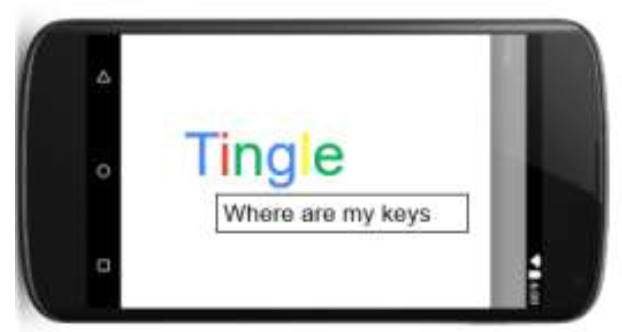
\includegraphics{images/FrontPage}

\begin{center}
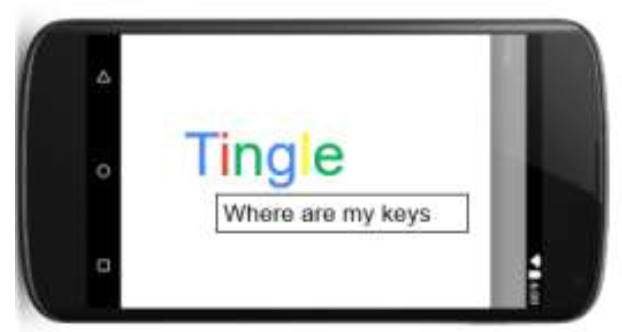
\includegraphics[width=\textwidth]{images/FrontPage}
\end{center}

\newpage

\tableofcontents

\newpage

% Report Content 

\section{Design choices}

% Introduction 

This chapter outlines some of the design choices that have been made throughout the course and iterative extension of the Tingle Application project. In particular, the MVC pattern and SOLID principles will be used to exemplify how parts of the Android project has been designed. Also, some of the main features including searching, sorting, camera, persistent storage and barcode lookup will be outlined as part of the major focus in the final version of the Tingle application. 

\subsection{MVC}

% Keywords: MVC, Package Diagram, explanation 

Firstly, I have separated the concerns of the software functionality by using the Model-View-Controller (MVC) design pattern (see package diagram in appendix \ref{App:AppendixA1}. The Views are composed of the XML layout files in the res layout package. Secondly, the Controllers are composed of the fragments, activities and widgets in the Controller package used to control the functionality of the views. Thirdly, the models are composed of the object-oriented domain classes in the Model package used to represent 'Thing' objects and hold the repository that defines how the application retrieves data from these objects. The MVC pattern has been used to avoid overlapping between the different functionalities of the program and thus achieve an overall modular design. Finally, yet another 'Helper' package has been used to hold classes that assist in providing some functionality that is not part of the overall MVC structure in the application (e.g. network, search and database functionality). 

\subsection{SOLID principles}

SOLID (single responsibility, open-closed, Liskov substitution, interface segregation and dependency inversion) is an acronym used in programming to describe five principles used within object-oriented programming and design in order to create a system that is easy to maintain and extend over time.\footnote{\url{https://en.wikipedia.org/wiki/SOLID_(object-oriented_design)} seen 23 April, 2016.} Some of the guidelines have been applied in this project to make the source code clear extensible, which is exemplified on the next page.

\subsubsection{Single Responsibility}

The single responsibility principle states that 'a class should only have one reason to change'. An example of this in the project would be the RecyclerView in 'ThingListFragment' and its adapter 'ThingAdapter'. The adapter is used to take the Thing data from the database and adapt it to a view in the RecyclerView. The adapter only has one responsibility which is to map a Thing object to its corresponding view that will be displayed on the screen within the list of items.

\noindent The onBindViewHolder method in the adapter is only responsible for the mapping from a Thing object to the view and does not perform any additional calculations. In this way, the Thing object and its calculation logic is not coupled to the adapter and we do not have to replicate any logic to display the Thing object elsewhere. 

\subsubsection{Open-closed}

The open-closed principle states that software entities (classes, modules, functions) should be open for extension but closed for modification. Basically, the existing code should not have to be changed every time the requirements change. An example of this would be the GenericSort abstract class and ISort interface used in the Search package. The GenericSort class outline the common features that all sorting algorithms should have (exchanging and comparing items) and the sorting calculation is abstracted away into an ISort interface with one responsibility defined - to sort Thing objects alphabetically based on their name or location. If you want to change the way items are sorted you simple extend (inherit) from GenericSort and implement the ISort interface to override the sorting method. As a result, duplicated code is avoided and the GenericSort class is kept open for extension but closed for modification.

\subsubsection{Liskov Substitution}

The Liskov Substitution principle states that the objects in a program should be replaceable with instances of their subtypes without altering the correctness of the program. By way of example, the Thing Repository needs a list of Things when retrieving data from the database in the getThings() method. The repository only requires that the list of things is of type List<Thing>. However, when we call the method we provide an ArrayList<Thing>. Since ArrayList<Thing> is a subtype of List<Thing> we are replacing the instance of the requested type (List<Thing>) with an instance of its subtype (ArrayList<Thing>). In other words, the code depends upon an abstraction and the program will run without any issues since the repository depends upon the contract provided by the List interface. In short, we can replace any list data structure that extends List and not break the program. 

\subsubsection{Interface Segregation}

The Interface Segregation principle states that the client should not be forced to depend upon interfaces that they don't use. This principle is sometimes violated in the project when implementing listeners on widgets used in the application UI. By way of example, the ViewPager class 'ThingPagerActivity' implements the onPageScrolled, onPageSelected and onPageScrollStateChanged listeners but only the first two of them are actually used. This leaves us with a 'fat interface' since we implement the full interface and provide dummy methods. Alternatively, one should provide many smaller interfaces to serve submodules in the project and avoid content in the interfaces that is not used. 

\subsubsection{Dependency Inversion}

The last Dependency Inversion principle states that the software entities should depend on abstractions rather than concretions. In other words, abstractions should not depend on details and details should depend upon abstractions. By way of example, an abstraction could be the IRepository interface used in the model package to outline the CRUD operations that the Thing Repository should support for retrieving data from the database. The direction of the dependency is 'inverted' by using interface contracts. In this case, the IRepository interface will reverse the direction of the data layer dependency and is instead put in the 'business layer'. The business objects only interact with the database via the high level interface. The data layer implements the repository interface – it contains concrete repositories which actually talk to the database. The dependency inversion maks unit testing possible since the domain objects now only depend on the IRepository interface that can be mocked or replaced with in-memory fake repositories. This has been violated to some degree in the project since a concrete Thing Repository is used in the controller classes to retrieve data.

\subsection{Fragments and Communication}

% Fragments, benefits, communication 

Fragments have been used to represent contents of the main page and list page UI since this could not be encapsulated to one activity UI component alone. For instance, the main page changes depending on the hardware configuration but this is not affected since each part of the UI is an independent fragment. Each fragment knows what they need to show and they do not communicate directly to each other. Instead, the fragments, 'TingleFragment' and 'ThingListFragment' communicate with their host activity, TingleActivity using a listener interface in the fragments that is implemented by the activity. Also, the fragment UI components are self-contained, modular and define their own layout and behaviour to allow reuse. The fragment captures the interface implementation during its onAttach() lifecycle method and can then call the interface methods in order to communicate with the activity. As opposed to using intents like in Tingle V3 where only activities were used. During runtime, the TingleActivity will receive events triggered from calling the interface method in the fragments (e.g. going back or showing the list of items). As a result, all Fragment-to-Fragment communication is done through the associated Activity and not directly. 

\subsection{Naming Conventions and Resources}

% Resources not hard coded, naming conventions for widgets and static objects 

Some of the conventions outlined in the book have been followed to uphold the guidelines within Android development. Specifically, the UI fields are denoted with 'm' naming conventions (e.g. "mButton") and string resource files are encapsulated in a separate XML file to avoid hard coding strings in the code (easy localization and cross language support). 

\subsection{New features}

Some of the new features introduced in the new version of Tingle 5 include search and sorting, camera pictures, barcode lookup and persistent storage in SQLite. All the functionalities have been implemented within classes in the Helper package. Specifically, the Search package holds the classes described previously in SOLID chapter and is used to allow the user to search and sort items based on their names and locations with the exception of the date that cannot be used to sort even though it is displayed as a menu item. The Database package contains new classes used to retrieve data from a SQLite database and uses a DatabaseManager class to create a thread-safe connection. Finally, the network package contains classes used to fetch data from item barcodes over the network using the Outpan API and AsyncTask to ensure that it happens on a background thread without affecting the UI. The camera functionality has been implemented using implicit intents to declare a general action to be performed allowing the built-in camera in the phone to be used to take a picture and register it with an item. Same goes for the barcode scanner that fires up the ZXing Barcode Scanner via an Intent. All together, these new features have been implemented to meet the minimum requirements of the final application.

\section{User Interface}
 
 % UI and widgets, hardware configuration, XML, custom menu bar items and launcher 
 
The User Interface is composed of the many XML layout files in the res layout package and include a layout for both portrait and landscape screen orientation. In this regard, I have chosen to make different layout files based on the orientation because some of the widgets are not relevant. By way of example, I do not include a Back button in the user interface composed in landscape mode. This is based on the fact that the main page is already shown in the fragment of the left container. Also, I do not include the "See Items" button used to redirect to the list of items in the ListFragment because they are already shown in landscape mode. Thus, I have designed the user interface for supporting both portrait and landscape orientation by using different layouts and widgets. 

\section{Testing}

\subsection{Manual Testing}
I have tested the application manually in an emulator on my computer and on a real Android device by adding things, flipping the phone, deleting things from the list, switching pages, scanning item barcodes and taking pictures. Manual testing was easy to do and gave me fast qualitative information on how my app behaved in different work flows. Specifically, I tested the usability (user experience), interface (testing of buttons) and compatibility (different screen sizes and orientations). Also, I have made some unit tests of the Model package to clarify that items are stored correctly and the underlying data logic layer works. I have chosen not to look into automated UI tests due to the relatively small complexity of the application so far. The manual testing combined with the unit tests of the model and repository allowed me to test all aspects of my app. However, I considered using the unit test framework 'Roboelectric' to remove the Android SDK and emulator dependency that makes running tests slow. 

\subsection{Test Sequences}

Below are some of the test sequences that have been used while manually testing the app. The test sequences cover important functionalities of the app (including error handling) and involve all parts of the user interface. Five test sequences have been included to cover the most essential use cases and functions. 

% Each & is a cell separator and the double-backslash \\ sets the end of this row

% Add new thing - Use Case 

\begin{center}
 \begin{tabular}{||c c c||} 
 \hline
 Use Case & Test Sequence & Result \\ [0.5ex] 
 \hline\hline
 Register thing & Start app in portrait mode. & Worked \\ 
 \hline
 & Fill name and location in text fields. & Worked \\
 \hline
 & Click scan button to register barcode. & Worked \\
 \hline
 & Fetch name from scanning item. & Worked \\
 \hline
 & Store thing information in SQLite database. & Worked \\
 \hline
 & Check that new thing is stored correctly. & Worked \\ [1ex] 
   \hline
\end{tabular}
\end{center}

% Search on thing - Use Case 

\begin{center}
 \begin{tabular}{||c c c||} 
 \hline
 Use Case & Test Sequence & Result \\ [0.5ex] 
 \hline\hline
 Search thing & Start app in portrait mode. & Worked \\ 
 \hline
 & Navigate to list of items by clicking 'See Items'. & Worked \\
 \hline
 & Click on search menu item. & Worked \\
 \hline
 & Type in search string and check for one hit. & Worked \\
 \hline
 & Type in search string and check for multiple hits. & Worked \\
 \hline
 & Type in search string and check for no hits. & Worked \\ [1ex] 
   \hline
\end{tabular}
\end{center}

% Delete thing(s) - Use Case 

\begin{center}
 \begin{tabular}{||c c c||} 
 \hline
 Use Case & Test Sequence & Result \\ [0.5ex] 
 \hline\hline
 Delete thing & Start app in portrait mode. & Worked \\ 
 \hline
 & Navigate to list of items by clicking 'See Items'. & Worked \\
 \hline
 & Long-tap item to activate multi selection. & Worked \\
 \hline
 & Select one item and delete. & Worked \\
 \hline
 & Select multiples items and delete. & Worked \\
 \hline
 & Try to delete item without long tap and multi select. & No delete \\
 \hline
 & Check that list is updated correctly. & Worked \\
 \hline
 & Check if item(s) are deleted from database. & Worked \\ [1ex] 
   \hline
\end{tabular}
\end{center}

% Scan thing - Use Case 

\begin{center}
 \begin{tabular}{||c c c||} 
 \hline
 Use Case & Test Sequence & Result \\ [0.5ex] 
 \hline\hline
 Scan barcode & Start app in portrait mode. & Worked \\ 
 \hline
 & Click 'Scan Item' and scan barcode. & Worked \\
 \hline
 & Check if barcode is inserted in barcode field. & Worked \\
 \hline
 & Wait for item name to be fetched from internet. & Worked \\
 \hline
 & Click 'Add New Thing'. & Worked \\
 \hline
 & Check if thing information is stored in database. & Worked \\ [1ex]
 \hline
\end{tabular}
\end{center}

% Take thing picture in detail page - Use Case 

\begin{center}
 \begin{tabular}{||c c c||} 
 \hline
 Use Case & Test Sequence & Result \\ [0.5ex] 
 \hline\hline
 Register Thing picture & Start app in portrait mode. & Worked \\ 
 \hline
 & Navigate to list of items by clicking 'See Items'. & Worked \\
 \hline
 & Navigate to item detail page by tapping item. & Worked \\
 \hline
 & Click camera button and take picture. & Work (not root) \\
 \hline
 & Check picture in image view and store item. & Worked \\
 \hline
 & Check if thing information is stored in database. & Worked \\ [1ex]
 \hline
\end{tabular}
\end{center}
 
% Exampels on manual test sequences including; 1) adding thing to database from portrait and landscape view, 2) searching and sorting list of items, 3) deleting one or multiple items from list using multi selection, 4) scanning a barcode and retrieving name using outpan, 5) taking a picture for a given item and storing it in detail view. 



\section{Problems}

% activities and fragments, screen choices, list performance vs sorting, Google API for location, camera intent on rooted phone , slow unit tests 

The main challenges in the Tingle version 4 were to replace the activities by fragments, associate the fragments through interfaces and most importantly to support different layouts based on the orientation of the device. A lot of time was spent on implementing the interfaces used to communicate between the fragments and the host activity while also moving the layout inflation in the onCreate() methods to the onCreateView() methods used in the fragments. Also, I had to make some deliberate choices about what to show on the screen based on the orientation (e.g. the back button was previously not shown in landscape mode). As opposed to Tingle version 4, a Scroll View has been used to fit all of the UI components in the detailed page and the landscape main page. This has allowed me to disregard the need to choose the most important UI components to be shown on the screen. Finally, one of the biggest problems introduced by the new features in version 5 derived from the searching and sorting functionality. The new functionality made it hard to update only specific parts of the list using notifyItemChanged(i) in the RecyclerView Adapter. By way of example, when the list of items is sorted all items may potentially swap positions and thus require the whole list to refresh using notifyDataSetChanged(). This also introduced an annoying bug when trying to delete items in a sorted list where items had changed their ViewHolder position, ultimately requiring a full refresh of the listcontent. Thus, the new version of Tingle has been designed to trade off some performance in return for the new search and sorting functionalities that allow the user to search and sort items based on their name and location. However, the extent of the list size has been judged to be relatively small with no real performance overhead added upon these changes. 

\iffalse

\section{Missing}
Test sequences (add item, delete item, multi and single selection, scan item, barcode lookup, search and sorting)
- New features (barcode scanner and lookup, sorting, multi search, camera, datepicker, maybe maps API)
- Go into depth with barcode lookup using stable network, camera using implicit intent and search using sorting and search algorithms 
- Optionally unit tests 
- Optionally enable location and maps to see where items were registered last 
- UML class and package diagram showing dependencies 
- UI Changes using custom logos and ScrollView to fit image view 

\fi

\newpage

% Bibliography with referenced sources 

\begin{thebibliography}{10}

% Course Book 

\bibitem{androidprogramming} 
Bill Phillips, Chris Stewart, Brian Hardy and Kristin Marsicano. 
\textit{Android Programming: The Big Nerd Ranch Guide}. 
Big Nerd Ranch, Reading, LLC, 2015.

% Algorithm book

\bibitem{algorithmsbook}
Robert Sedgewick and Kevin Wayne.
\textit{Algorithms, 4th Edition}.
Princeton University, Addison-Wesley, 2011.

% Android Developer Links 

\bibitem{fragmentcommunication}
Android Developer: Communicating With Other Fragments, 
retrieved on April 23, 2016 from \url{http://developer.android.com/training/basics/fragments/communicating.html} 

\bibitem{network}
Android Developer: Connecting To The Network, 
retrieved on April 23, 2016 from \url{http://developer.android.com/training/basics/network-ops/connecting.html} 

\bibitem{threads}
Android Developer: Processes and Threads, 
retrieved on April 23, 2016 from \url{http://developer.android.com/guide/components/processes-and-threads.html} 

\bibitem{services}
Android Developer: Services, 
retrieved on April 23, 2016 from \url{http://developer.android.com/guide/components/services.html
}

\bibitem{bitmaps}
Android Developer: Loading Large Bitmaps Efficientlys, 
retrieved on April 23, 2016 from \url{http://developer.android.com/training/displaying-bitmaps/load-bitmap.html} 

\bibitem{androidintents}
Vogella: Android Intents, 
\emph{Vogella}, 2014 Lars Vogel, 
retrieved on April 23, 2016 from \url{http://www.vogella.com/tutorials/AndroidIntent/article.html} 

\bibitem{androidtesting}
Big Nerd Ranch: Testing the Android way, 
\emph{Big Nerd Ranch}, 2016 Josh Skeen, 
retrieved on April 23, 2016 from \url {https://www.bignerdranch.com/blog/testing-the-android-way/}

% Other links 

\bibitem{multiseletion}
Big Nerd Ranch: RecyclerView MultiSelect, 
\emph{The MIT Licence}, 2014 Big Nerd Ranch
retrieved on April 23, 2016 from \url {http://bignerdranch.github.io/recyclerview-multiselect/}

\bibitem{selectionsort}
Princeton University: SelectionSort Source Code, 
\emph{The MIT Licence}, 2010 Robert Sedgewick and Kevin Wayne, 
retrieved on April 23, 2016 from \url {http://algs4.cs.princeton.edu/21elementary/Selection.java.html}

\bibitem{zxing}
ZXing Barcode Scanner, 
\emph{Apache License}, 2004 RZXing, 
retrieved on April 23, 2016 from \url {https://github.com/zxing/zxing}


\end{thebibliography}

% \ref{fig:mainpagePortrait} Reference example 

\newpage





 
\appendix
\section{Appendices}
  
% UML diagrams
  
\subsection{Tingle Package Diagram} \label{App:AppendixA1}

\begin{figure}[h!]
	\centering
	\includegraphics[scale=0.7]{"/UMLLucidChart/PackageDiagram"}
	\caption{UML Package Diagram}
	\label{fig:packagediagram}
\end{figure}

\newpage

\subsection{Tingle View Class Diagram} \label{App:AppendixA2}

\begin{figure}[h!]
	\centering
	\includegraphics[scale=0.7]{"/UMLLucidChart/ViewClassDiagram"}
	\caption{UML View Class Diagram}
	\label{fig:viewclassdiagram}
\end{figure}

\newpage

\subsection{Tingle Model Class Diagram} \label{App:AppendixA3}

\begin{figure}[h!]
	\centering
	\includegraphics[scale=0.2]{"/UMLLucidChart/ModelClassDiagram"}
	\caption{UML Model Class Diagram}
	\label{fig:modelclassdiagram}
\end{figure}

\newpage

\subsection{Tingle Controller Class Diagram} \label{App:AppendixA4}

\begin{figure}[h!]
	\centering
	\includegraphics[scale=0.6]{"/UMLLucidChart/ControllerClassDiagram"}
	\caption{UML Controller Class Diagram}
	\label{fig:controllerclassdiagram}
\end{figure}

\newpage

\subsection{Tingle Component Subsystem Diagram} \label{App:AppendixA5}

\begin{figure}[h!]
	\centering
	\includegraphics[scale=0.3]{"/UMLLucidChart/ComponentSubsystemDiagram"}
	\caption{UML Component Subsystem Diagram}
	\label{fig:componentsubsystemdiagram}
\end{figure}

\newpage

% UI 

\subsection{Tingle App Main Page UI} \label{App:AppendixA6}

\begin{figure}[h!]
	\centering
	\includegraphics[scale=0.7]{"/UI/TingleHomePage"}
	\caption{Main page in portrait mode}
	\label{fig:mainpageportrait}
\end{figure}

\newpage

\subsection{Tingle App Landscape Main Page UI} \label{App:AppendixA7}

\begin{figure}[h!]
	\centering
	\includegraphics[scale=0.7]{"/UI/Landscape"}
	\caption{Main page in landscape mode}
	\label{fig:mainpagelandscape}
\end{figure}

\newpage

\subsection{Tingle List Page UI} \label{App:AppendixA8}

\begin{figure}[h!]
	\centering
	\includegraphics[scale=0.7]{"/UI/TingleListPage"}
	\caption{List page}
	\label{fig:listpage}
\end{figure}

\newpage

\subsection{Tingle Search and Sorting Menu Items UI} \label{App:AppendixA9}

\begin{figure}[h!]
	\centering
	\includegraphics[scale=0.7]{"/UI/Sorting"}
	\caption{List page}
	\label{fig:listpage}
\end{figure}

\newpage

\subsection{Tingle Detailed Page UI} \label{App:AppendixA10}

\begin{figure}[h!]
	\centering
	\includegraphics[scale=0.7]{"/UI/TingleDetailedPage"}
	\caption{Detailed page}
	\label{fig:detailpage}
\end{figure}


	
\end{document}